\chapter{Methodology} \label{chap:methodology}

In this chapter, we present the development of a visual servoing method based on using the trifocal tensor elements as visual features in our visual servoing control loop. We begin by developing the needed control law using the tensor, finding the respective interaction matrix, and then exploring the normalization approach for the obtained tensor and interaction matrix. Finally we represent the overall procedure for the proposed algorithm to be implemented.

\section{Control Law}
To formulate the control law of the trifocal tensor based visual servoing, we need to establish the model of the system and find the relation between the input of the control and the trifocal tensor coefficients. The trifocal tensor can be computed from feature correspondences across the three views. Our goal is to find the interaction matrix relating the control input and the tensor derivatives.
\begin{equation}
  \dot{\mathcal{T}}_{(jkl)} = L_{\mathcal{T}_{(jkl)}} \begin{pmatrix} v_c \\ w_c \end{pmatrix}
\end{equation}

\subsection{Coefficients of the Trifocal Tensor}
To compute the relation between the coefficients of the trifocal tensor and the Projective matrices, first we write the Tensor relation \eqref{eq:trifocalgeometry1} with the proper visual servoing notation as follows
\begin{equation}
  \mathcal{T}_{(jkl)} = a_{(kj)}b_{(4l)} - a_{(4k)}b_{(lj)} \label{eq:tensorrelation}
\end{equation}

For the sake of maintaining the Visual Servoing convention, we omit the use of $i$ as an index for the tensor relation. The letter $i$ further on will be indicating the initial view in the control system. The Camera positions are then written as $C_{c^*},C_c,C_i$ for the desired, current, and initial camera positions respectively. The same may also be done for the projection matrices, and instead of using the matrices $A,B$ to express the homography between the first and second or third views, we will use the standard notation from Visual Servoing with the corresponding Rotation matrices $^{c}R_{c^*}, ^{i}R_{c^*}$ respectively. For the translations $a_4, b_4$, we will use $^{c}{t}_{c^*}, ^{i}{t}_{c^*}$ respectively. Leading superscripts will denote the frame with respect to which a set of coordinates are defined. Thus, the rotation matrix $^{c}R_{c^*}$ gives the orientation of the desired camera frame relative to the current camera frame.

\begin{align*}
  C &\Rightarrow C_{c^*} \text{  Desired camera position} \\
  C' &\Rightarrow C_c \text{  Current camera position} \\
  C^{''} &\Rightarrow C_i \text{  Initial camera position} \\
\end{align*}
\begin{gather*}
  P_d = P = [I | 0]\\
  P_c = P^{\prime} = [A | a_4] : ^{c}{\bf M}_{c^*} = [ ^{c}{\bf R}_{c^*} | ^{c}{\bf t}_{c^*} ]\\
  P_i = P^{\prime \prime} = [B | b_4] : ^{i}{\bf M}_{c^*} = [ ^{i}{\bf R}_{c^*} | ^{i}{\bf t}_{c^*} ]
\end{gather*}

The Tensor relation \eqref{eq:tensorrelation} can then be expressed as follows
\begin{equation}
\mathcal{T}_{(jkl)} = \tensor[^{c}]{R}{_{c^{*}(kj)}} \ \tensor[^{i}]{t}{_{c^{*}(l)}} - \tensor[^{c}]{t}{_{c^{*}(k)}} \ \tensor[^{i}]{R}{_{c^{*}(lj)}} \label{eq:tensorcoeffs}
\end{equation}

Expanding this relation further to compute the tensor coefficients is straight forward, expanding for values of $j,k,l$ we get the following tensor coefficients:

\begin{equation}
\begin{gathered}
  \mathcal{T}_{(111)} = \tensor[^{c}]{R}{_{c^{*}(11)}} \ \tensor[^{i}]{t}{_{c^{*}(1)}} - \tensor[^{c}]{t}{_{c^{*}(1)}} \ \tensor[^{i}]{R}{_{c^{*}(11)}}\\
  \mathcal{T}_{(112)} = \tensor[^{c}]{R}{_{c^{*}(11)}} \ \tensor[^{i}]{t}{_{c^{*}(2)}} - \tensor[^{c}]{t}{_{c^{*}(1)}} \ \tensor[^{i}]{R}{_{c^{*}(21)}}\\
  \mathcal{T}_{(113)} = \tensor[^{c}]{R}{_{c^{*}(11)}} \ \tensor[^{i}]{t}{_{c^{*}(3)}} - \tensor[^{c}]{t}{_{c^{*}(1)}} \ \tensor[^{i}]{R}{_{c^{*}(31)}}\\
  \mathcal{T}_{(121)} = \tensor[^{c}]{R}{_{c^{*}(21)}} \ \tensor[^{i}]{t}{_{c^{*}(1)}} - \tensor[^{c}]{t}{_{c^{*}(2)}} \ \tensor[^{i}]{R}{_{c^{*}(11)}}\\
  \mathcal{T}_{(122)} = \tensor[^{c}]{R}{_{c^{*}(21)}} \ \tensor[^{i}]{t}{_{c^{*}(2)}} - \tensor[^{c}]{t}{_{c^{*}(2)}} \ \tensor[^{i}]{R}{_{c^{*}(21)}}\\
  \mathcal{T}_{(123)} = \tensor[^{c}]{R}{_{c^{*}(21)}} \ \tensor[^{i}]{t}{_{c^{*}(3)}} - \tensor[^{c}]{t}{_{c^{*}(2)}} \ \tensor[^{i}]{R}{_{c^{*}(31)}}\\
  \mathcal{T}_{(131)} = \tensor[^{c}]{R}{_{c^{*}(31)}} \ \tensor[^{i}]{t}{_{c^{*}(1)}} - \tensor[^{c}]{t}{_{c^{*}(3)}} \ \tensor[^{i}]{R}{_{c^{*}(11)}}\\
  \mathcal{T}_{(132)} = \tensor[^{c}]{R}{_{c^{*}(31)}} \ \tensor[^{i}]{t}{_{c^{*}(2)}} - \tensor[^{c}]{t}{_{c^{*}(3)}} \ \tensor[^{i}]{R}{_{c^{*}(21)}}\\
  \mathcal{T}_{(133)} = \tensor[^{c}]{R}{_{c^{*}(31)}} \ \tensor[^{i}]{t}{_{c^{*}(3)}} - \tensor[^{c}]{t}{_{c^{*}(3)}} \ \tensor[^{i}]{R}{_{c^{*}(31)}}\\
  \mathcal{T}_{(211)} = \tensor[^{c}]{R}{_{c^{*}(12)}} \ \tensor[^{i}]{t}{_{c^{*}(1)}} - \tensor[^{c}]{t}{_{c^{*}(1)}} \ \tensor[^{i}]{R}{_{c^{*}(12)}}\\
  \mathcal{T}_{(212)} = \tensor[^{c}]{R}{_{c^{*}(12)}} \ \tensor[^{i}]{t}{_{c^{*}(2)}} - \tensor[^{c}]{t}{_{c^{*}(1)}} \ \tensor[^{i}]{R}{_{c^{*}(22)}}\\
  \mathcal{T}_{(213)} = \tensor[^{c}]{R}{_{c^{*}(12)}} \ \tensor[^{i}]{t}{_{c^{*}(3)}} - \tensor[^{c}]{t}{_{c^{*}(1)}} \ \tensor[^{i}]{R}{_{c^{*}(32)}}\\
  \mathcal{T}_{(221)} = \tensor[^{c}]{R}{_{c^{*}(22)}} \ \tensor[^{i}]{t}{_{c^{*}(1)}} - \tensor[^{c}]{t}{_{c^{*}(2)}} \ \tensor[^{i}]{R}{_{c^{*}(12)}}\\
  \mathcal{T}_{(222)} = \tensor[^{c}]{R}{_{c^{*}(22)}} \ \tensor[^{i}]{t}{_{c^{*}(2)}} - \tensor[^{c}]{t}{_{c^{*}(2)}} \ \tensor[^{i}]{R}{_{c^{*}(22)}}\\
  \mathcal{T}_{(223)} = \tensor[^{c}]{R}{_{c^{*}(22)}} \ \tensor[^{i}]{t}{_{c^{*}(3)}} - \tensor[^{c}]{t}{_{c^{*}(2)}} \ \tensor[^{i}]{R}{_{c^{*}(32)}}\\
  \mathcal{T}_{(231)} = \tensor[^{c}]{R}{_{c^{*}(32)}} \ \tensor[^{i}]{t}{_{c^{*}(1)}} - \tensor[^{c}]{t}{_{c^{*}(3)}} \ \tensor[^{i}]{R}{_{c^{*}(12)}}\\
  \mathcal{T}_{(232)} = \tensor[^{c}]{R}{_{c^{*}(32)}} \ \tensor[^{i}]{t}{_{c^{*}(2)}} - \tensor[^{c}]{t}{_{c^{*}(3)}} \ \tensor[^{i}]{R}{_{c^{*}(22)}}\\
  \mathcal{T}_{(233)} = \tensor[^{c}]{R}{_{c^{*}(32)}} \ \tensor[^{i}]{t}{_{c^{*}(3)}} - \tensor[^{c}]{t}{_{c^{*}(3)}} \ \tensor[^{i}]{R}{_{c^{*}(32)}}\\
  \mathcal{T}_{(311)} = \tensor[^{c}]{R}{_{c^{*}(13)}} \ \tensor[^{i}]{t}{_{c^{*}(1)}} - \tensor[^{c}]{t}{_{c^{*}(1)}} \ \tensor[^{i}]{R}{_{c^{*}(13)}}\\
  \mathcal{T}_{(312)} = \tensor[^{c}]{R}{_{c^{*}(13)}} \ \tensor[^{i}]{t}{_{c^{*}(2)}} - \tensor[^{c}]{t}{_{c^{*}(1)}} \ \tensor[^{i}]{R}{_{c^{*}(23)}}\\
  \mathcal{T}_{(313)} = \tensor[^{c}]{R}{_{c^{*}(13)}} \ \tensor[^{i}]{t}{_{c^{*}(3)}} - \tensor[^{c}]{t}{_{c^{*}(1)}} \ \tensor[^{i}]{R}{_{c^{*}(33)}}\\
  \mathcal{T}_{(321)} = \tensor[^{c}]{R}{_{c^{*}(23)}} \ \tensor[^{i}]{t}{_{c^{*}(1)}} - \tensor[^{c}]{t}{_{c^{*}(2)}} \ \tensor[^{i}]{R}{_{c^{*}(13)}}\\
  \mathcal{T}_{(322)} = \tensor[^{c}]{R}{_{c^{*}(23)}} \ \tensor[^{i}]{t}{_{c^{*}(2)}} - \tensor[^{c}]{t}{_{c^{*}(2)}} \ \tensor[^{i}]{R}{_{c^{*}(23)}}\\
  \mathcal{T}_{(323)} = \tensor[^{c}]{R}{_{c^{*}(23)}} \ \tensor[^{i}]{t}{_{c^{*}(3)}} - \tensor[^{c}]{t}{_{c^{*}(2)}} \ \tensor[^{i}]{R}{_{c^{*}(33)}}\\
  \mathcal{T}_{(331)} = \tensor[^{c}]{R}{_{c^{*}(33)}} \ \tensor[^{i}]{t}{_{c^{*}(1)}} - \tensor[^{c}]{t}{_{c^{*}(3)}} \ \tensor[^{i}]{R}{_{c^{*}(13)}}\\
  \mathcal{T}_{(332)} = \tensor[^{c}]{R}{_{c^{*}(33)}} \ \tensor[^{i}]{t}{_{c^{*}(2)}} - \tensor[^{c}]{t}{_{c^{*}(3)}} \ \tensor[^{i}]{R}{_{c^{*}(23)}}\\
  \mathcal{T}_{(333)} = \tensor[^{c}]{R}{_{c^{*}(33)}} \ \tensor[^{i}]{t}{_{c^{*}(3)}} - \tensor[^{c}]{t}{_{c^{*}(3)}} \ \tensor[^{i}]{R}{_{c^{*}(33)}}
\end{gathered}\label{eq:tensorcoeffsexpanded}
\end{equation}

\pagebreak

Our objective is to move our robot from the initial camera position to the desired target camera position. Therefore, we have two special cases for the tensor coefficients values.
\begin{description}
  \item[First when $C_c$ at the initial position $C_i$] \hfill
    \begin{equation}
    \begin{gathered}
      \tensor[^{c}]{R}{_{c^{*}}} = \tensor[^{i}]{R}{_{c^{*}}}, \ \tensor[^{c}]{t}{_{c^{*}}} = \tensor[^{i}]{t}{_{c^{*}}}\\
      \mathcal{T}_{(jkl)}^{i} = \tensor[^{c}]{R}{_{c^{*}(kj)}} \ \tensor[^{c}]{t}{_{c^{*}(l)}} - \tensor[^{c}]{t}{_{c^{*}(k)}} \ \tensor[^{c}]{R}{_{c^{*}(lj)}}\\
      \text{when } k = l, \mathcal{T}_{(jkl)}^{i} = 0\\
      \mathcal{T}_{(112)}^{i} = -\mathcal{T}_{(121)}^{i}, \mathcal{T}_{(113)}^{i} = -\mathcal{T}_{(131)}^{i}, \mathcal{T}_{(123)}^{i} = -\mathcal{T}_{(132)}^{i}\\
      \mathcal{T}_{(212)}^{i} = -\mathcal{T}_{(221)}^{i}, \mathcal{T}_{(213)}^{i} = -\mathcal{T}_{(231)}^{i}, \mathcal{T}_{(223)}^{i} = -\mathcal{T}_{(232)}^{i}\\
      \mathcal{T}_{(312)}^{i} = -\mathcal{T}_{(321)}^{i}, \mathcal{T}_{(313)}^{i} = -\mathcal{T}_{(331)}^{i}, \mathcal{T}_{(323)}^{i} = -\mathcal{T}_{(332)}^{i}
    \end{gathered}\label{eq:tensorcoeffinitial}
    \end{equation}
  \item[Second when $C_c$ at the desired position $C_{c^*}$] \hfill
    \begin{equation}
    \begin{gathered}
      \tensor[^{c}]{R}{_{c^{*}}} = I, \ \tensor[^{c}]{t}{_{c^{*}}} = \bf{0}\\
      \mathcal{T}_{(jkl)}^{*} = I_{(kj)} \ \tensor[^{i}]{t}{_{c^{*}(l)}}\\
      \text{when } j \neq k, \mathcal{T}_{(jkl)}^{*} = 0\\
      \mathcal{T}_{(111)}^{*} = \mathcal{T}_{(221)}^{*} = \mathcal{T}_{(331)}^{*} = \tensor[^{i}]{t}{_{c^{*}(1)}}\\
      \mathcal{T}_{(112)}^{*} = \mathcal{T}_{(222)}^{*} = \mathcal{T}_{(332)}^{*} = \tensor[^{i}]{t}{_{c^{*}(2)}}\\
      \mathcal{T}_{(113)}^{*} = \mathcal{T}_{(223)}^{*} = \mathcal{T}_{(333)}^{*} = \tensor[^{i}]{t}{_{c^{*}(3)}}
    \end{gathered}\label{eq:tensorcoeffdesired}
  \end{equation}
\end{description}

\subsection{Tensor Derivation}
\label{sub:tensor_derivation}

First, The derivatives of all the trifocal tensor elements with respect to time are generally as following:
\begin{equation}
  \dot{\mathcal{T}}_{(jkl)} = \tensor[^{c}]{\dot{R}}{_{c^{*}(kj)}} \ \tensor[^{i}]{t}{_{c^{*}(l)}} + \tensor[^{c}]{R}{_{c^{*}(kj)}} \ \tensor[^{i}]{\dot{t}}{_{c^{*}(l)}} - \tensor[^{c}]{\dot{t}}{_{c^{*}(k)}} \ \tensor[^{i}]{R}{_{c^{*}(lj)}} - \tensor[^{c}]{t}{_{c^{*}(k)}} \ \tensor[^{i}]{\dot{R}}{_{c^{*}(lj)}} \label{eq:tensorderivatives1}
\end{equation}

Since our initial camera $C_i$ is fixed, the elements of the derivatives of its rotation matrix and its transpose vector are equal to zero, \textit{i.e.:} $\tensor[^i]{\dot{t}}{_{c^{*}(l)}} = \tensor[^i]{\dot{R}}{_{c^{*}(jl)}} = 0$. Our trifocal tensor elements derivative is then simplified to:
\begin{equation}
  \dot{\mathcal{T}}_{(jkl)} = \tensor[^{c}]{\dot{R}}{_{c^{*}(kj)}} \ \tensor[^{i}]{t}{_{c^{*}(l)}} - \tensor[^{c}]{\dot{t}}{_{c^{*}(k)}} \ \tensor[^{i}]{R}{_{c^{*}(lj)}} \label{eq:tensorderivatives2}
\end{equation}

The spatial velocity of the camera is $u_c = {(v_c, \omega_{c})}^{T}$, where $v_c$ and $\omega_c$ are the translational and rotational velocities of the camera. From the geometry of the scene, we can deduce the following relationships:
\begin{gather*}
  {[\omega_{c}]}_{\times} = \tensor[^{c^*}]{R}{_{c}^{T}} \tensor[^{c^*}]{\dot{R}}{_{c}} = - \tensor[^{c^*}]{\dot{R}}{_{c}^{T}} \tensor[^{c^*}]{R}{_{c}}\\
  \tensor[^{c^*}]{\dot{R}}{_{c}^{T}} = - {[\omega_{c}]}_{\times}\tensor[^{c^*}]{R}{_{c}^{T}}\\
  \tensor[^{c^*}]{\dot{R}}{_{c}^{T}} = - {[\omega_{c}]}_{\times}\tensor[^{c}]{R}{_{c^*}}\\
  \tensor[^{c}]{\dot{R}}{_{c^*}} = -{[\omega_c]}_{\times}\tensor[^{c}]{R}{_{c^*}}\\
  %
  \tensor[^{c^*}]{\dot{t}}{_{c}} = \tensor[^{c^*}]{R}{_{c}}v_{c}\\
  \tensor[^{c}]{t}{_{c^*}} = - \tensor[^{c}]{R}{_{c^*}} \tensor[^{c^*}]{t}{_{c}}\\
  \tensor[^{c}]{\dot{t}}{_{c^*}} = - \tensor[^{c}]{\dot{R}}{_{c^*}} \tensor[^{c^*}]{t}{_{c}} - \tensor[^{c}]{R}{_{c^*}} \tensor[^{c^*}]{\dot{t}}{_{c}}\\
  \tensor[^{c}]{\dot{t}}{_{c^*}} = {[\omega_c]}_{\times}\tensor[^{c}]{R}{_{c^*}} \tensor[^{c^*}]{t}{_{c}} - \tensor[^{c}]{R}{_{c^*}} \tensor[^{c^*}]{R}{_{c}}v_{c}\\
  \tensor[^{c}]{\dot{t}}{_{c^*}} = {[\omega_c]}_{\times}\tensor[^{c}]{t}{_{c^*}} - v_{c}\\
  \tensor[^{c}]{\dot{t}}{_{c^*}} = {[\tensor[^{c}]{t}{_{c^*}}]}_{\times}\omega_c - v_{c}\\
%
  \tensor[^{c}]{\dot{t}}{_{c^{*}(k)}} = [-I | {[\tensor[^{c}]{t}{_{c^*}}]}_{\times}] u
\end{gather*}

Substituting back into the tensor derivation \eqref{eq:tensorderivatives2}, we get:
\begin{equation}
\begin{gathered}
  \dot{\mathcal{T}}_{(jkl)} =  - {({[\omega_c]}_{\times}\tensor[^{c}]{R}{_{c^*}})}_{(kj)}\ \tensor[^{i}]{t}{_{c^*(l)}} - {({[\tensor[^{c}]{t}{_{c^*}}]}_{\times}\omega_c - v_{c})}_{(k)}\ \tensor[^{i}]{R}{_{c^*(lj)}}\\
  \dot{\mathcal{T}}_{(jkl)} =  - (\sum_{m}{[\omega_{c}]}_{\times(km)}\tensor[^{c}]{R}{_{c^*(mj)}})\ \tensor[^{i}]{t}{_{c^*(l)}} - ({({[\tensor[^{c}]{t}{_{c^*}}]}_{\times}\omega_c)}_{(k)}  -   v_{c(k)})\ \tensor[^{i}]{R}{_{c^*(lj)}}
\end{gathered}\label{eq:tensorderivatives3}
\end{equation}

where
\begin{gather*}
\tensor[^{i}]{t}{_{c^*}} = -\tensor[^{i}]{R}{_{c^*}}\begin{pmatrix} x_i \\ y_i \\ z_i \end{pmatrix}, \
\tensor[^{c}]{t}{_{c^*}} = -\tensor[^{c}]{R}{_{c^*}}\begin{pmatrix} x_c \\ y_c \\ z_c \end{pmatrix}, \\
  \tensor[^{i}]{R}{_{c^*}} = \begin{bmatrix}
    R_{i(11)} & R_{i(12)} & R_{i(13)} \\
    R_{i(21)} & R_{i(22)} & R_{i(23)} \\
    R_{i(31)} & R_{i(32)} & R_{i(33)}
  \end{bmatrix},\
\tensor[^{c}]{R}{_{c^*}} = \begin{bmatrix}
  R_{c(11)} & R_{c(12)} & R_{c(13)} \\
  R_{c(21)} & R_{c(22)} & R_{c(23)} \\
  R_{c(31)} & R_{c(32)} & R_{c(33)}
\end{bmatrix},\\
{[\omega_{c}]}_{\times} = \begin{bmatrix} 0 & -\omega_z & \omega_y \\ \omega_z & 0 & -\omega_y \\ -\omega_y & \omega_x & 0 \end{bmatrix},\
{[\tensor[^{c}]{t}{_{c^*}}]}_{\times}\omega_c  = \begin{bmatrix} -\tensor[^{c}]{t}{_{c^*(3)}}\omega_y + \tensor[^{c}]{t}{_{c^*(2)}} \omega_z \\\ \ \tensor[^{c}]{t}{_{c^*(3)}}\omega_x - \tensor[^{c}]{t}{_{c^*(1)}} \omega_z \\ -\tensor[^{c}]{t}{_{c^*(2)}}\omega_x + \tensor[^{c}]{t}{_{c^*(1)}}\omega_y \end{bmatrix}
\end{gather*}

From~\eqref{eq:tensorcoeffsexpanded} and~\eqref{eq:tensorderivatives3}, the derivative of the first tensor coefficient can be computed as follows:
\begin{equation}
\begin{gathered}
  \dot{\mathcal{T}}_{(111)} =  - (-R_{c(21)} \omega_z + R_{c(31)}\omega_y)\ \tensor[^{i}]{t}{_{c^*(1)}} - (-\tensor[^{c}]{t}{_{c^*(3)}}\omega_y + \tensor[^{c}]{t}{_{c^*(2)}} \omega_z - v_x)\ \tensor[^{i}]{R}{_{c^*(11)}}\\
  \dot{\mathcal{T}}_{(111)} = R_{i(11)}v_x - (R_{c(31)}\tensor[^{i}]{t}{_{c^*(1)}} - R_{i(11)}\tensor[^{c}]{t}{_{c^*(3)}}) \omega_y  + (R_{c(21)}\tensor[^{i}]{t}{_{c^*(1)}} - R_{i(11)}\tensor[^{c}]{t}{_{c^*(2)}} ) \omega_z\\
  \dot{\mathcal{T}}_{(111)} = R_{i(11)}v_x - \mathcal{T}_{(131)} \omega_y  +  \mathcal{T}_{(121)} \omega_z
\end{gathered}
\end{equation}

By expanding the derivatives for the rest of the coefficients, we can deduce this compact form for the tensor coefficients derivatives:
\begin{equation}
\begin{gathered}
  \dot{\mathcal{T}}_{(jkl)} = R_{i(lj)}v_{c(k)} - \sum_{m} {[\omega_{c}]}_{\times(km)} \mathcal{T}_{(jml)}
%%  \dot{\mathcal{T}}_{(111)} =  - (-R_{c(21)} \omega_z + R_{c(31)}\omega_y)\ \tensor[^{i}]{t}{_{c^*(1)}} - (-\tensor[^{c}]{t}{_{c^*(3)}}\omega_y + \tensor[^{c}]{t}{_{c^*(2)}} \omega_z -v_x)\ \tensor[^{i}]{R}{_{c^*(11)}}\\
%%  \dot{\mathcal{T}}_{(112)} =  - (-R_{c(21)} \omega_z + R_{c(31)}\omega_y)\ \tensor[^{i}]{t}{_{c^*(2)}} - (-\tensor[^{c}]{t}{_{c^*(3)}}\omega_y + \tensor[^{c}]{t}{_{c^*(2)}} \omega_z -v_x)\ \tensor[^{i}]{R}{_{c^*(21)}}\\
%%  \dot{\mathcal{T}}_{(113)} =  - (-R_{c(21)} \omega_z + R_{c(31)}\omega_y)\ \tensor[^{i}]{t}{_{c^*(3)}} - (-\tensor[^{c}]{t}{_{c^*(3)}}\omega_y + \tensor[^{c}]{t}{_{c^*(2)}} \omega_z -v_x)\ \tensor[^{i}]{R}{_{c^*(31)}}\\
%%  %
%%  \dot{\mathcal{T}}_{(121)} =  - ( R_{c(11)} \omega_z - R_{c(31)}\omega_x)\ \tensor[^{i}]{t}{_{c^*(1)}} - ( \tensor[^{c}]{t}{_{c^*(3)}}\omega_x - \tensor[^{c}]{t}{_{c^*(1)}} \omega_z -v_y)\ \tensor[^{i}]{R}{_{c^*(11)}}\\
%%  \dot{\mathcal{T}}_{(122)} =  - ( R_{c(11)} \omega_z - R_{c(31)}\omega_x)\ \tensor[^{i}]{t}{_{c^*(2)}} - ( \tensor[^{c}]{t}{_{c^*(3)}}\omega_x - \tensor[^{c}]{t}{_{c^*(1)}} \omega_z -v_y)\ \tensor[^{i}]{R}{_{c^*(21)}}\\
%%  \dot{\mathcal{T}}_{(123)} =  - ( R_{c(11)} \omega_z - R_{c(w1)}\omega_x)\ \tensor[^{i}]{t}{_{c^*(3)}} - ( \tensor[^{c}]{t}{_{c^*(3)}}\omega_x - \tensor[^{c}]{t}{_{c^*(1)}} \omega_z -v_y)\ \tensor[^{i}]{R}{_{c^*(31)}}\\
%%  %
%%  \dot{\mathcal{T}}_{(131)} =  - (-R_{c(11)} \omega_y + R_{c(21)}\omega_x)\ \tensor[^{i}]{t}{_{c^*(1)}} - (-\tensor[^{c}]{t}{_{c^*(2)}}\omega_x + \tensor[^{c}]{t}{_{c^*(1)}} \omega_y -v_z)\ \tensor[^{i}]{R}{_{c^*(11)}}\\
%%  \dot{\mathcal{T}}_{(132)} =  - (-R_{c(11)} \omega_y + R_{c(21)}\omega_x)\ \tensor[^{i}]{t}{_{c^*(2)}} - (-\tensor[^{c}]{t}{_{c^*(2)}}\omega_x + \tensor[^{c}]{t}{_{c^*(1)}} \omega_y -v_z)\ \tensor[^{i}]{R}{_{c^*(21)}}\\
%%  \dot{\mathcal{T}}_{(133)} =  - (-R_{c(11)} \omega_y + R_{c(21)}\omega_x)\ \tensor[^{i}]{t}{_{c^*(3)}} - (-\tensor[^{c}]{t}{_{c^*(2)}}\omega_x + \tensor[^{c}]{t}{_{c^*(1)}} \omega_y -v_z)\ \tensor[^{i}]{R}{_{c^*(31)}}\\
%%  %
%%  %
%%  \dot{\mathcal{T}}_{(211)} =  - (-R_{c(22)} \omega_z + R_{c(32)}\omega_y)\ \tensor[^{i}]{t}{_{c^*(1)}} - (-\tensor[^{c}]{t}{_{c^*(3)}}\omega_y + \tensor[^{c}]{t}{_{c^*(2)}} \omega_z -v_x)\ \tensor[^{i}]{R}{_{c^*(12)}}\\
%%  \dot{\mathcal{T}}_{(212)} =  - (-R_{c(22)} \omega_z + R_{c(32)}\omega_y)\ \tensor[^{i}]{t}{_{c^*(2)}} - (-\tensor[^{c}]{t}{_{c^*(3)}}\omega_y + \tensor[^{c}]{t}{_{c^*(2)}} \omega_z -v_x)\ \tensor[^{i}]{R}{_{c^*(22)}}\\
%%  \dot{\mathcal{T}}_{(213)} =  - (-R_{c(22)} \omega_z + R_{c(32)}\omega_y)\ \tensor[^{i}]{t}{_{c^*(3)}} - (-\tensor[^{c}]{t}{_{c^*(3)}}\omega_y + \tensor[^{c}]{t}{_{c^*(2)}} \omega_z -v_x)\ \tensor[^{i}]{R}{_{c^*(32)}}\\
%%  %
%%  \dot{\mathcal{T}}_{(221)} =  - ( R_{c(12)} \omega_z - R_{c(32)}\omega_x)\ \tensor[^{i}]{t}{_{c^*(1)}} - ( \tensor[^{c}]{t}{_{c^*(3)}}\omega_x - \tensor[^{c}]{t}{_{c^*(1)}} \omega_z -v_y)\ \tensor[^{i}]{R}{_{c^*(12)}}\\
%%  \dot{\mathcal{T}}_{(222)} =  - ( R_{c(12)} \omega_z - R_{c(32)}\omega_x)\ \tensor[^{i}]{t}{_{c^*(2)}} - ( \tensor[^{c}]{t}{_{c^*(3)}}\omega_x - \tensor[^{c}]{t}{_{c^*(1)}} \omega_z -v_y)\ \tensor[^{i}]{R}{_{c^*(22)}}\\
%%  \dot{\mathcal{T}}_{(223)} =  - ( R_{c(12)} \omega_z - R_{c(w2)}\omega_x)\ \tensor[^{i}]{t}{_{c^*(3)}} - ( \tensor[^{c}]{t}{_{c^*(3)}}\omega_x - \tensor[^{c}]{t}{_{c^*(1)}} \omega_z -v_y)\ \tensor[^{i}]{R}{_{c^*(32)}}\\
%%  %
%%  \dot{\mathcal{T}}_{(231)} =  - (-R_{c(12)} \omega_y + R_{c(22)}\omega_x)\ \tensor[^{i}]{t}{_{c^*(1)}} - (-\tensor[^{c}]{t}{_{c^*(2)}}\omega_x + \tensor[^{c}]{t}{_{c^*(1)}} \omega_y -v_z)\ \tensor[^{i}]{R}{_{c^*(12)}}\\
%%  \dot{\mathcal{T}}_{(232)} =  - (-R_{c(12)} \omega_y + R_{c(22)}\omega_x)\ \tensor[^{i}]{t}{_{c^*(2)}} - (-\tensor[^{c}]{t}{_{c^*(2)}}\omega_x + \tensor[^{c}]{t}{_{c^*(1)}} \omega_y -v_z)\ \tensor[^{i}]{R}{_{c^*(22)}}\\
%%  \dot{\mathcal{T}}_{(233)} =  - (-R_{c(12)} \omega_y + R_{c(22)}\omega_x)\ \tensor[^{i}]{t}{_{c^*(3)}} - (-\tensor[^{c}]{t}{_{c^*(2)}}\omega_x + \tensor[^{c}]{t}{_{c^*(1)}} \omega_y -v_z)\ \tensor[^{i}]{R}{_{c^*(32)}}\\
%%  %
%%  %
%%  \dot{\mathcal{T}}_{(311)} =  - (-R_{c(23)} \omega_z + R_{c(33)}\omega_y)\ \tensor[^{i}]{t}{_{c^*(1)}} - (-\tensor[^{c}]{t}{_{c^*(3)}}\omega_y + \tensor[^{c}]{t}{_{c^*(2)}} \omega_z -v_x)\ \tensor[^{i}]{R}{_{c^*(13)}}\\
%%  \dot{\mathcal{T}}_{(312)} =  - (-R_{c(23)} \omega_z + R_{c(33)}\omega_y)\ \tensor[^{i}]{t}{_{c^*(2)}} - (-\tensor[^{c}]{t}{_{c^*(3)}}\omega_y + \tensor[^{c}]{t}{_{c^*(2)}} \omega_z -v_x)\ \tensor[^{i}]{R}{_{c^*(23)}}\\
%%  \dot{\mathcal{T}}_{(313)} =  - (-R_{c(23)} \omega_z + R_{c(33)}\omega_y)\ \tensor[^{i}]{t}{_{c^*(3)}} - (-\tensor[^{c}]{t}{_{c^*(3)}}\omega_y + \tensor[^{c}]{t}{_{c^*(2)}} \omega_z -v_x)\ \tensor[^{i}]{R}{_{c^*(33)}}\\
%%  %
%%  \dot{\mathcal{T}}_{(321)} =  - ( R_{c(13)} \omega_z - R_{c(33)}\omega_x)\ \tensor[^{i}]{t}{_{c^*(1)}} - ( \tensor[^{c}]{t}{_{c^*(3)}}\omega_x - \tensor[^{c}]{t}{_{c^*(1)}} \omega_z -v_y)\ \tensor[^{i}]{R}{_{c^*(13)}}\\
%%  \dot{\mathcal{T}}_{(322)} =  - ( R_{c(13)} \omega_z - R_{c(33)}\omega_x)\ \tensor[^{i}]{t}{_{c^*(2)}} - ( \tensor[^{c}]{t}{_{c^*(3)}}\omega_x - \tensor[^{c}]{t}{_{c^*(1)}} \omega_z -v_y)\ \tensor[^{i}]{R}{_{c^*(23)}}\\
%%  \dot{\mathcal{T}}_{(323)} =  - ( R_{c(13)} \omega_z - R_{c(w3)}\omega_x)\ \tensor[^{i}]{t}{_{c^*(3)}} - ( \tensor[^{c}]{t}{_{c^*(3)}}\omega_x - \tensor[^{c}]{t}{_{c^*(1)}} \omega_z -v_y)\ \tensor[^{i}]{R}{_{c^*(33)}}\\
%%  %
%%  \dot{\mathcal{T}}_{(331)} =  - (-R_{c(13)} \omega_y + R_{c(23)}\omega_x)\ \tensor[^{i}]{t}{_{c^*(1)}} - (-\tensor[^{c}]{t}{_{c^*(2)}}\omega_x + \tensor[^{c}]{t}{_{c^*(1)}} \omega_y -v_z)\ \tensor[^{i}]{R}{_{c^*(13)}}\\
%%  \dot{\mathcal{T}}_{(332)} =  - (-R_{c(13)} \omega_y + R_{c(23)}\omega_x)\ \tensor[^{i}]{t}{_{c^*(2)}} - (-\tensor[^{c}]{t}{_{c^*(2)}}\omega_x + \tensor[^{c}]{t}{_{c^*(1)}} \omega_y -v_z)\ \tensor[^{i}]{R}{_{c^*(23)}}\\
%%  \dot{\mathcal{T}}_{(333)} =  - (-R_{c(13)} \omega_y + R_{c(23)}\omega_x)\ \tensor[^{i}]{t}{_{c^*(3)}} - (-\tensor[^{c}]{t}{_{c^*(2)}}\omega_x + \tensor[^{c}]{t}{_{c^*(1)}} \omega_y -v_z)\ \tensor[^{i}]{R}{_{c^*(33)}}\\
\end{gathered}\label{eq:tensorderivativesgeneral}
\end{equation}

\subsection{Interaction Matrix}
\label{sub:interaction_matrix}
To control the six degrees of freedom, at least six tensor coefficients are necessary. However, to avoid singularities, more than six tensor coefficients are considered. The interaction matrix taking into account all the tensor coefficients is given in~\eqref{eq:interactionmatrix}. It is important to notice that pose of the initial camera location is necessary for the computation of the interaction matrix as well as the normalization factor. This initial pose can be retrieved by computing the equivalent projection matrix for the estimated trifocal tensor as show in~\ref{sub:recovering_projection_matrices}. This step is done at the control loop initialization.

\begin{equation}
\begin{gathered}
 L_{\mathcal{T}_{(jkl)}} = %\frac{1}{\mathcal{T}_{N}}
  \begin{bmatrix}
      \tensor[^{i}]{R}{_{c^*(11)}} & 0 & 0 & 0 & - \mathcal{T}_{(131)} & \mathcal{T}_{(121)}\\
      \tensor[^{i}]{R}{_{c^*(21)}} & 0 & 0 & 0 & - \mathcal{T}_{(132)} & \mathcal{T}_{(122)}\\
      \tensor[^{i}]{R}{_{c^*(31)}} & 0 & 0 & 0 & - \mathcal{T}_{(133)} & \mathcal{T}_{(123)}\\

      0 & \tensor[^{i}]{R}{_{c^*(11)}} & 0 & \mathcal{T}_{(131)} & 0 & - \mathcal{T}_{(111)}\\
      0 & \tensor[^{i}]{R}{_{c^*(21)}} & 0 & \mathcal{T}_{(132)} & 0 & - \mathcal{T}_{(112)}\\
      0 & \tensor[^{i}]{R}{_{c^*(31)}} & 0 & \mathcal{T}_{(133)} & 0 & - \mathcal{T}_{(113)}\\

      0 & 0 & \tensor[^{i}]{R}{_{c^*(11)}} & - \mathcal{T}_{(121)} & \mathcal{T}_{(111)} & 0 \\
      0 & 0 & \tensor[^{i}]{R}{_{c^*(21)}} & - \mathcal{T}_{(122)} & \mathcal{T}_{(112)} & 0 \\
      0 & 0 & \tensor[^{i}]{R}{_{c^*(31)}} & - \mathcal{T}_{(123)} & \mathcal{T}_{(113)} & 0 \\


      \tensor[^{i}]{R}{_{c^*(12)}} & 0 & 0 & 0 & - \mathcal{T}_{(231)} & \mathcal{T}_{(221)}\\
      \tensor[^{i}]{R}{_{c^*(22)}} & 0 & 0 & 0 & - \mathcal{T}_{(232)} & \mathcal{T}_{(222)}\\
      \tensor[^{i}]{R}{_{c^*(32)}} & 0 & 0 & 0 & - \mathcal{T}_{(233)} & \mathcal{T}_{(223)}\\

      0 & \tensor[^{i}]{R}{_{c^*(12)}} & 0 & \mathcal{T}_{(231)} & 0 & - \mathcal{T}_{(211)}\\
      0 & \tensor[^{i}]{R}{_{c^*(22)}} & 0 & \mathcal{T}_{(232)} & 0 & - \mathcal{T}_{(212)}\\
      0 & \tensor[^{i}]{R}{_{c^*(32)}} & 0 & \mathcal{T}_{(233)} & 0 & - \mathcal{T}_{(213)}\\

      0 & 0 & \tensor[^{i}]{R}{_{c^*(12)}} & - \mathcal{T}_{(221)} & \mathcal{T}_{(211)} & 0 \\
      0 & 0 & \tensor[^{i}]{R}{_{c^*(22)}} & - \mathcal{T}_{(222)} & \mathcal{T}_{(212)} & 0 \\
      0 & 0 & \tensor[^{i}]{R}{_{c^*(32)}} & - \mathcal{T}_{(223)} & \mathcal{T}_{(213)} & 0 \\


      \tensor[^{i}]{R}{_{c^*(13)}} & 0 & 0 & 0 & - \mathcal{T}_{(331)} & \mathcal{T}_{(321)}\\
      \tensor[^{i}]{R}{_{c^*(23)}} & 0 & 0 & 0 & - \mathcal{T}_{(332)} & \mathcal{T}_{(322)}\\
      \tensor[^{i}]{R}{_{c^*(33)}} & 0 & 0 & 0 & - \mathcal{T}_{(333)} & \mathcal{T}_{(323)}\\

      0 & \tensor[^{i}]{R}{_{c^*(13)}} & 0 & \mathcal{T}_{(331)} & 0 & - \mathcal{T}_{(311)}\\
      0 & \tensor[^{i}]{R}{_{c^*(23)}} & 0 & \mathcal{T}_{(332)} & 0 & - \mathcal{T}_{(312)}\\
      0 & \tensor[^{i}]{R}{_{c^*(33)}} & 0 & \mathcal{T}_{(333)} & 0 & - \mathcal{T}_{(313)}\\

      0 & 0 & \tensor[^{i}]{R}{_{c^*(13)}} & - \mathcal{T}_{(321)} & \mathcal{T}_{(311)} & 0 \\
      0 & 0 & \tensor[^{i}]{R}{_{c^*(23)}} & - \mathcal{T}_{(322)} & \mathcal{T}_{(312)} & 0 \\
      0 & 0 & \tensor[^{i}]{R}{_{c^*(33)}} & - \mathcal{T}_{(323)} & \mathcal{T}_{(313)} & 0
  \end{bmatrix}
\end{gathered}\label{eq:interactionmatrix}
\end{equation}

When the camera reach the desired position, the interaction matrix is as follows:
\begin{equation}
\begin{gathered}
  L_{\mathcal{T}^{*}_{(jkl)}} = %\frac{1}{\mathcal{T}_{N}}
  \begin{bmatrix}
      \tensor[^{i}]{R}{_{c^*(11)}} & 0 & 0 & 0 & 0 &0\\
      \tensor[^{i}]{R}{_{c^*(21)}} & 0 & 0 & 0 & 0 &0\\
      \tensor[^{i}]{R}{_{c^*(31)}} & 0 & 0 & 0 & 0 &0\\

      0 & \tensor[^{i}]{R}{_{c^*(11)}} & 0 & 0 & 0 & - \tensor[^{i}]{t}{_{c^*(1)}}\\
      0 & \tensor[^{i}]{R}{_{c^*(21)}} & 0 & 0 & 0 & - \tensor[^{i}]{t}{_{c^*(2)}}\\
      0 & \tensor[^{i}]{R}{_{c^*(31)}} & 0 & 0 & 0 & - \tensor[^{i}]{t}{_{c^*(3)}}\\

      0 & 0 & \tensor[^{i}]{R}{_{c^*(11)}} & 0 & \tensor[^{i}]{t}{_{c^*(1)}} & 0 \\
      0 & 0 & \tensor[^{i}]{R}{_{c^*(21)}} & 0 & \tensor[^{i}]{t}{_{c^*(2)}} & 0 \\
      0 & 0 & \tensor[^{i}]{R}{_{c^*(31)}} & 0 & \tensor[^{i}]{t}{_{c^*(3)}} & 0 \\


      \tensor[^{i}]{R}{_{c^*(12)}} & 0 & 0 & 0 & 0 & \tensor[^{i}]{t}{_{c^*(1)}}\\
      \tensor[^{i}]{R}{_{c^*(22)}} & 0 & 0 & 0 & 0 & \tensor[^{i}]{t}{_{c^*(2)}}\\
      \tensor[^{i}]{R}{_{c^*(32)}} & 0 & 0 & 0 & 0 & \tensor[^{i}]{t}{_{c^*(3)}}\\

      0 & \tensor[^{i}]{R}{_{c^*(12)}} & 0 & 0 & 0 & 0\\
      0 & \tensor[^{i}]{R}{_{c^*(22)}} & 0 & 0 & 0 & 0\\
      0 & \tensor[^{i}]{R}{_{c^*(32)}} & 0 & 0 & 0 & 0\\

      0 & 0 & \tensor[^{i}]{R}{_{c^*(12)}} & - \tensor[^{i}]{t}{_{c^*(1)}} & 0 & 0 \\
      0 & 0 & \tensor[^{i}]{R}{_{c^*(22)}} & - \tensor[^{i}]{t}{_{c^*(2)}} & 0 & 0 \\
      0 & 0 & \tensor[^{i}]{R}{_{c^*(32)}} & - \tensor[^{i}]{t}{_{c^*(3)}} & 0 & 0 \\


      \tensor[^{i}]{R}{_{c^*(13)}} & 0 & 0 & 0 & - \tensor[^{i}]{t}{_{c^*(1)}} &0\\
      \tensor[^{i}]{R}{_{c^*(23)}} & 0 & 0 & 0 & - \tensor[^{i}]{t}{_{c^*(2)}} &0\\
      \tensor[^{i}]{R}{_{c^*(33)}} & 0 & 0 & 0 & - \tensor[^{i}]{t}{_{c^*(3)}} &0\\

      0 & \tensor[^{i}]{R}{_{c^*(13)}} & 0 & \tensor[^{i}]{t}{_{c^*(1)}} & 0 & 0\\
      0 & \tensor[^{i}]{R}{_{c^*(23)}} & 0 & \tensor[^{i}]{t}{_{c^*(2)}} & 0 & 0\\
      0 & \tensor[^{i}]{R}{_{c^*(33)}} & 0 & \tensor[^{i}]{t}{_{c^*(3)}} & 0 & 0\\

      0 & 0 & \tensor[^{i}]{R}{_{c^*(13)}} & 0 & 0 & 0 \\
      0 & 0 & \tensor[^{i}]{R}{_{c^*(23)}} & 0 & 0 & 0 \\
      0 & 0 & \tensor[^{i}]{R}{_{c^*(33)}} & 0 & 0 & 0
  \end{bmatrix}
\end{gathered}\label{eq:interactionmatrixdesired}
\end{equation}
\subsection{Tensor Normalization}
\label{sub:tensor_normalization}
In this approach, no metric information, depth estimation or trifocal tensor decomposition were used. Hence, we need to define a common scale of the trifocal tensor for the control law. The trifocal tensor is normalized to get a fixed scale with $\mathcal{T}_{N}$. When the camera reaches the desired goal position, we can observe from~\eqref{eq:tensorcoeffdesired} that the tensor coefficients are only related to the translation of the camera at the initial position which is a constant value vector. Also from~\eqref{eq:interactionmatrix}, the first column elements $\mathcal{T}_{(111)}$, $\mathcal{T}_{(112)}$, $\mathcal{T}_{(113)}$, $\mathcal{T}_{(211)}$, $\mathcal{T}_{(212)}$, $\mathcal{T}_{(213)}$, $\mathcal{T}_{(311)}$, $\mathcal{T}_{(312)}$, $\mathcal{T}_{(313)}$ are respectively equal to $\tensor[^{i}]{t}{_{c^*(1)}}$, $\tensor[^{i}]{t}{_{c^*(2)}}$, $\tensor[^{i}]{t}{_{c^*(3)}}$, $0$,$0$,$0$,$0$,$0$,$0$ at the desired goal position.

Choosing the elements $\mathcal{T}_{(111)}$, $\mathcal{T}_{(112)}$, $\mathcal{T}_{(113)}$ as normalization factor, we can normalize the elements $T_{jkl}$ for $k = 1$ as follows:

%Thus, the norm of the vector $\lVert \tensor[^{i}]{t}{_{c^*}} \rVert$ can be used as a normalization factor for the trifocal tensor. Then the normalized trifocal tensor coefficients are:
\begin{equation}
  \begin{gathered}
    T_{jkl} = \frac{\mathcal{T}_{jkl}}{\mathcal{T}_{1N}}\\
    \mathcal{T}_{1N} = \sqrt{{\mathcal{T}_{111}}^{2}+{\mathcal{T}_{112}}^{2}+{\mathcal{T}_{113}}^{2}}\\
    \dot{\mathcal{T}}_{1N} = \frac{1}{\sqrt{{\mathcal{T}_{111}}^{2}+{\mathcal{T}_{112}}^{2}+{\mathcal{T}_{113}}^{2}}}(\mathcal{T}_{111}\dot{\mathcal{T}}_{111} + \mathcal{T}_{112}\dot{\mathcal{T}}_{112} + \mathcal{T}_{113}\dot{\mathcal{T}}_{113})\\
    \dot{\mathcal{T}}_{1N} = \frac{1}{\mathcal{T}_{N}}(\mathcal{T}_{111}\dot{\mathcal{T}}_{111} + \mathcal{T}_{112}\dot{\mathcal{T}}_{112} + \mathcal{T}_{113}\dot{\mathcal{T}}_{113})\\
    \dot{\mathcal{T}}_{1N} = \frac{1}{\mathcal{T}_{N}}(\mathcal{T}_{111}(R_{i(11)} v_x - \mathcal{T}_{131} \omega_y + \mathcal{T}_{121} \omega_z) \\+ \mathcal{T}_{112}(R_{i(21)} v_x - \mathcal{T}_{132} \omega_y + \mathcal{T}_{122} \omega_z) + \mathcal{T}_{113}(R_{i(31)} v_x - \mathcal{T}_{133} \omega_y + \mathcal{T}_{123} \omega_z))\\
  \dot{\mathcal{T}}_{1N} = \begin{bmatrix}T_{111}R_{i(11)} + T_{112}R_{i(21)} + T_{113}R_{i(31)} \\ 0 \\ 0 \\ 0 \\ -T_{111}\mathcal{T}_{131} - T_{112}\mathcal{T}_{132} - T_{113}\mathcal{T}_{133} \\  T_{111}\mathcal{T}_{121} + T_{112}\mathcal{T}_{122} + T_{113}\mathcal{T}_{123}\end{bmatrix}^{T} u_c\\
    \dot{\mathcal{T}}_{1N} = L_{1N} u_c\\
    \\
    \dot{T}_{jkl} = \frac{\dot{\mathcal{T}}_{jkl}}{\mathcal{T}_{N}} - \frac{\mathcal{T}_{jkl} \dot{\mathcal{T}_{N}}}{{\mathcal{T}_{N}}^{2}}\\
    \dot{T}_{jkl} = \frac{L_{\mathcal{T}} u_c}{\mathcal{T}_{N}} - \frac{\mathcal{T}_{jkl} L_{N} u_c}{{\mathcal{T}_{N}}^{2}}\\
    \dot{T}_{jkl} = \frac{L_{\mathcal{T}} u_c}{\mathcal{T}_{N}} - \frac{T_{jkl} L_{N} u_c}{{\mathcal{T}_{N}}}\\
    \dot{T}_{jkl} = \frac{1}{\mathcal{T}_{N}} (L_{\mathcal{T}} - T_{jkl} L_{N}) u_c\\
    L_{T} = \frac{1}{\mathcal{T}_{N}} (L_{\mathcal{T}} - T_{jkl} L_{N})\\
    L_{1T} = \frac{L_{1\mathcal{T}}}{\mathcal{T}_{1N}} - T_{j1l} \begin{bmatrix}T_{111}\frac{R_{i(11)}}{\mathcal{T}_{1N}} + T_{112}\frac{R_{i(21)}}{\mathcal{T}_{1N}} + T_{113}\frac{R_{i(31)}}{\mathcal{T}_{1N}} \\ 0 \\ 0 \\ 0 \\ -T_{111}T_{131} - T_{112}T_{132} - T_{113}T_{133} \\  T_{111}T_{121} + T_{112}T_{122} + T_{113}T_{123}\end{bmatrix}^{T}\\
    \dot{T}_{(j1l)} = \frac{R_{i(lj)}}{\mathcal{T}_{1N}}v_{c(1)} -T_{(j1l)}(T_{111}\frac{R_{i(11)}}{\mathcal{T}_{1N}} + T_{112}\frac{R_{i(21)}}{\mathcal{T}_{1N}} + T_{113}\frac{R_{i(31)}}{\mathcal{T}_{1N}}) v_{c(1)}\\ + T_{(j1l)}(T_{111}T_{131} + T_{112}T_{132} + T_{113}T_{133})\omega_y - T_{(j1l)}(T_{111}T_{121} + T_{112}T_{122} + T_{113}T_{123})\omega_z \\+\sum_{m} {[\omega_{c}]}_{\times(1m)} T_{(jml)}\\
  %L_{T(jkl)} = \begin{bmatrix}\frac{R_{i(11)}}{\mathcal{T}_{N}} -T_{(jkl)}(T_{111}\frac{R_{i(11)}}{\mathcal{T}_{N}} + T_{112}\frac{R_{i(21)}}{\mathcal{T}_{N}} + T_{113}\frac{R_{i(31)}}{\mathcal{T}_{N}}) \\ 0 \\ 0 \\ 0 \\ - T_{(131)} + T_{(jkl)}(T_{111}T_{131} + T_{112}T_{132} + T_{113}T_{133}) \\ T_{(121)} - T_{(jkl)}(T_{111}T_{121} + T_{112}T_{122} + T_{113}T_{123})\end{bmatrix}\\
  \end{gathered}\label{eq:tensornormalizationk1}
\end{equation}
%
%The use of the initial camera position is conveniant in visual servoing as the normalization factor $\mathcal{T}_{N}$ is never equal to zero except when the initial and desired camera positions are the same, which is not valid in our context. Also, this normalization factor is constant with time and doesn't affect the tensor derivatives. The trifocal tensor estimation is then computed relative to the initial camera position distance which can be estimated in the initialization step and used further for the control loop.
Same approach can be applied again for the rest of the elemtns for $k= 2,3$:
\begin{equation}
  \begin{gathered}
    T_{j2l} = \frac{\mathcal{T}_{j2l}}{\mathcal{T}_{2N}}\\
    \mathcal{T}_{2N} = \sqrt{{\mathcal{T}_{221}}^{2}+{\mathcal{T}_{222}}^{2}+{\mathcal{T}_{223}}^{2}}\\
    \dot{\mathcal{T}}_{2N} = \frac{1}{\sqrt{{\mathcal{T}_{221}}^{2}+{\mathcal{T}_{222}}^{2}+{\mathcal{T}_{223}}^{2}}}(\mathcal{T}_{221}\dot{\mathcal{T}}_{221} + \mathcal{T}_{222}\dot{\mathcal{T}}_{222} + \mathcal{T}_{223}\dot{\mathcal{T}}_{223})\\
    \dot{\mathcal{T}}_{2N} = \frac{1}{\mathcal{T}_{2N}}(\mathcal{T}_{221}\dot{\mathcal{T}}_{221} + \mathcal{T}_{222}\dot{\mathcal{T}}_{222} + \mathcal{T}_{223}\dot{\mathcal{T}}_{223})\\
    \dot{\mathcal{T}}_{2N} = \frac{1}{\mathcal{T}_{2N}}(\mathcal{T}_{221}(R_{i(12)} v_y - \mathcal{T}_{231} \omega_x + \mathcal{T}_{211} \omega_z) \\+ \mathcal{T}_{222}(R_{i(22)} v_y - \mathcal{T}_{232} \omega_x + \mathcal{T}_{212} \omega_z) + \mathcal{T}_{223}(R_{i(32)} v_y - \mathcal{T}_{233} \omega_x + \mathcal{T}_{213} \omega_z))\\
  \dot{\mathcal{T}}_{2N} = \begin{bmatrix}0 \\ T_{221}R_{i(12)} + T_{222}R_{i(22)} + T_{223}R_{i(32)} \\ 0 \\  T_{221}\mathcal{T}_{231} + T_{222}\mathcal{T}_{232} + T_{223}\mathcal{T}_{233} \\ 0 \\ -T_{221}\mathcal{T}_{211} - T_{222}\mathcal{T}_{212} - T_{223}\mathcal{T}_{213}\end{bmatrix}^{T} u_c\\
    \dot{\mathcal{T}}_{3N} = \begin{bmatrix}0 \\ 0 \\ T_{331}R_{i(13)} + T_{332}R_{i(23)} + T_{333}R_{i(33)} \\  -T_{331}\mathcal{T}_{321} - T_{332}\mathcal{T}_{322} - T_{333}\mathcal{T}_{323} \\ T_{331}\mathcal{T}_{311} + T_{332}\mathcal{T}_{312} + T_{333}\mathcal{T}_{313} \\ 0\end{bmatrix}^{T} u_c\\
    \\
    \dot{T}_{(jkl)} = \frac{R_{i(lj)}}{\mathcal{T}_{kN}}v_{c(k)} -T_{(jkl)}(\sum_{m}T_{kkm}\frac{R_{i(mk)}}{\mathcal{T}_{kN}}) v_{c(k)}\\ + T_{(jkl)}(\sum_{m}T_{kkm}T_{khm})\omega_{(g)} - T_{(jkl)}(\sum_{m}T_{kkm}T_{kgm})\omega_{(h)} \\+\sum_{m} {[\omega_{c}]}_{\times(km)} T_{(jml)}\\
      \text{where } g = k\%3 +1, h = (k+1)\%3 +1
  \end{gathered}\label{eq:tensornormalizationk23}
\end{equation}

\begin{landscape}
Normalized Interaction Matrix
\begin{equation}
\begin{gathered}
% L_{\mathcal{T}_{(jkl)}} = %\frac{1}{\mathcal{T}_{N}}
  \scalemath{0.70}{
  \begin{bmatrix}
    \frac{R_{i(11)}}{\mathcal{T}_{N}} -T_{(111)}(\sum_{m}T_{11m}\frac{R_{i(m1)}}{\mathcal{T}_{1N}}) & 0 & 0 & 0 & - T_{(131)} + T_{(111)}(\sum_{m}T_{11m}T_{13m}) & T_{(121)}- T_{(111)}(\sum_{m}T_{11m}T_{12m})\\
    \frac{R_{i(21)}}{\mathcal{T}_{N}} -T_{(112)}(\sum_{m}T_{11m}\frac{R_{i(m1)}}{\mathcal{T}_{1N}}) & 0 & 0 & 0 & - T_{(132)} + T_{(112)}(\sum_{m}T_{11m}T_{13m}) & T_{(122)}- T_{(112)}(\sum_{m}T_{11m}T_{12m})\\
    \frac{R_{i(31)}}{\mathcal{T}_{N}} -T_{(113)}(\sum_{m}T_{11m}\frac{R_{i(m1)}}{\mathcal{T}_{1N}}) & 0 & 0 & 0 & - T_{(133)} + T_{(113)}(\sum_{m}T_{11m}T_{13m}) & T_{(123)}- T_{(113)}(\sum_{m}T_{11m}T_{12m})\\

    0 & \frac{R_{i(11)}}{\mathcal{T}_{N}} -T_{(121)}(\sum_{m}T_{22m}\frac{R_{i(m2)}}{\mathcal{T}_{2N}}) & 0 & T_{(131)} - T_{(121)}(\sum_{m}T_{22m}T_{23m})& 0 & - T_{(111)}+ T_{(121)}(\sum_{m}T_{22m}T_{21m})\\
    0 & \frac{R_{i(21)}}{\mathcal{T}_{N}} -T_{(122)}(\sum_{m}T_{22m}\frac{R_{i(m2)}}{\mathcal{T}_{2N}}) & 0 & T_{(132)} - T_{(122)}(\sum_{m}T_{22m}T_{23m})& 0 & - T_{(112)}+ T_{(122)}(\sum_{m}T_{22m}T_{21m})\\
    0 & \frac{R_{i(31)}}{\mathcal{T}_{N}} -T_{(123)}(\sum_{m}T_{22m}\frac{R_{i(m2)}}{\mathcal{T}_{2N}}) & 0 & T_{(133)} - T_{(123)}(\sum_{m}T_{22m}T_{23m})& 0 & - T_{(113)}+ T_{(123)}(\sum_{m}T_{22m}T_{21m})\\

    0 & 0 & \frac{R_{i(11)}}{\mathcal{T}_{N}} -T_{(131)}(\sum_{m}T_{33m}\frac{R_{i(m3)}}{\mathcal{T}_{3N}}) & - T_{(121)} + T_{(131)}(\sum_{m}T_{33m}T_{32m}) & T_{(111)} - T_{(131)}(\sum_{m}T_{33m}T_{31m})& 0 \\
    0 & 0 & \frac{R_{i(21)}}{\mathcal{T}_{N}} -T_{(132)}(\sum_{m}T_{33m}\frac{R_{i(m3)}}{\mathcal{T}_{3N}}) & - T_{(122)} + T_{(132)}(\sum_{m}T_{33m}T_{32m}) & T_{(112)} - T_{(132)}(\sum_{m}T_{33m}T_{31m})& 0 \\
    0 & 0 & \frac{R_{i(31)}}{\mathcal{T}_{N}} -T_{(133)}(\sum_{m}T_{33m}\frac{R_{i(m3)}}{\mathcal{T}_{3N}}) & - T_{(123)} + T_{(133)}(\sum_{m}T_{33m}T_{32m}) & T_{(113)} - T_{(133)}(\sum_{m}T_{33m}T_{31m})& 0 \\


    \frac{R_{i(12)}}{\mathcal{T}_{N}} -T_{(211)}(\sum_{m}T_{11m}\frac{R_{i(m1)}}{\mathcal{T}_{1N}}) & 0 & 0 & 0 & - T_{(231)} + T_{(211)}(\sum_{m}T_{11m}T_{13m}) & T_{(221)}- T_{(211)}(\sum_{m}T_{11m}T_{12m})\\
    \frac{R_{i(22)}}{\mathcal{T}_{N}} -T_{(212)}(\sum_{m}T_{11m}\frac{R_{i(m1)}}{\mathcal{T}_{1N}}) & 0 & 0 & 0 & - T_{(232)} + T_{(212)}(\sum_{m}T_{11m}T_{13m}) & T_{(222)}- T_{(212)}(\sum_{m}T_{11m}T_{12m})\\
    \frac{R_{i(32)}}{\mathcal{T}_{N}} -T_{(213)}(\sum_{m}T_{11m}\frac{R_{i(m1)}}{\mathcal{T}_{1N}}) & 0 & 0 & 0 & - T_{(233)} + T_{(213)}(\sum_{m}T_{11m}T_{13m}) & T_{(223)}- T_{(213)}(\sum_{m}T_{11m}T_{12m})\\

    0 & \frac{R_{i(12)}}{\mathcal{T}_{N}} -T_{(221)}(\sum_{m}T_{22m}\frac{R_{i(m2)}}{\mathcal{T}_{2N}}) & 0 & T_{(231)} - T_{(221)}(\sum_{m}T_{22m}T_{23m})& 0 & - T_{(211)}+ T_{(221)}(\sum_{m}T_{22m}T_{21m})\\
    0 & \frac{R_{i(22)}}{\mathcal{T}_{N}} -T_{(222)}(\sum_{m}T_{22m}\frac{R_{i(m2)}}{\mathcal{T}_{2N}}) & 0 & T_{(232)} - T_{(222)}(\sum_{m}T_{22m}T_{23m})& 0 & - T_{(212)}+ T_{(222)}(\sum_{m}T_{22m}T_{21m})\\
    0 & \frac{R_{i(32)}}{\mathcal{T}_{N}} -T_{(223)}(\sum_{m}T_{22m}\frac{R_{i(m2)}}{\mathcal{T}_{2N}}) & 0 & T_{(233)} - T_{(223)}(\sum_{m}T_{22m}T_{23m})& 0 & - T_{(213)}+ T_{(223)}(\sum_{m}T_{22m}T_{21m})\\

    0 & 0 & \frac{R_{i(12)}}{\mathcal{T}_{N}} -T_{(231)}(\sum_{m}T_{33m}\frac{R_{i(m3)}}{\mathcal{T}_{3N}}) & - T_{(221)} + T_{(231)}(\sum_{m}T_{33m}T_{32m}) & T_{(211)} - T_{(231)}(\sum_{m}T_{33m}T_{31m})& 0 \\
    0 & 0 & \frac{R_{i(22)}}{\mathcal{T}_{N}} -T_{(232)}(\sum_{m}T_{33m}\frac{R_{i(m3)}}{\mathcal{T}_{3N}}) & - T_{(222)} + T_{(232)}(\sum_{m}T_{33m}T_{32m}) & T_{(212)} - T_{(232)}(\sum_{m}T_{33m}T_{31m})& 0 \\
    0 & 0 & \frac{R_{i(32)}}{\mathcal{T}_{N}} -T_{(233)}(\sum_{m}T_{33m}\frac{R_{i(m3)}}{\mathcal{T}_{3N}}) & - T_{(223)} + T_{(233)}(\sum_{m}T_{33m}T_{32m}) & T_{(213)} - T_{(233)}(\sum_{m}T_{33m}T_{31m})& 0 \\


    \frac{R_{i(13)}}{\mathcal{T}_{N}} -T_{(311)}(\sum_{m}T_{11m}\frac{R_{i(m1)}}{\mathcal{T}_{1N}}) & 0 & 0 & 0 & - T_{(331)} + T_{(311)}(\sum_{m}T_{11m}T_{13m}) & T_{(321)}- T_{(311)}(\sum_{m}T_{11m}T_{12m})\\
    \frac{R_{i(23)}}{\mathcal{T}_{N}} -T_{(312)}(\sum_{m}T_{11m}\frac{R_{i(m1)}}{\mathcal{T}_{1N}}) & 0 & 0 & 0 & - T_{(332)} + T_{(312)}(\sum_{m}T_{11m}T_{13m}) & T_{(322)}- T_{(312)}(\sum_{m}T_{11m}T_{12m})\\
    \frac{R_{i(33)}}{\mathcal{T}_{N}} -T_{(313)}(\sum_{m}T_{11m}\frac{R_{i(m1)}}{\mathcal{T}_{1N}}) & 0 & 0 & 0 & - T_{(333)} + T_{(313)}(\sum_{m}T_{11m}T_{13m}) & T_{(323)}- T_{(313)}(\sum_{m}T_{11m}T_{12m})\\

    0 & \frac{R_{i(13)}}{\mathcal{T}_{N}} -T_{(321)}(\sum_{m}T_{22m}\frac{R_{i(m2)}}{\mathcal{T}_{2N}}) & 0 & T_{(331)} - T_{(321)}(\sum_{m}T_{22m}T_{23m})& 0 & - T_{(311)}+ T_{(321)}(\sum_{m}T_{22m}T_{21m})\\
    0 & \frac{R_{i(23)}}{\mathcal{T}_{N}} -T_{(322)}(\sum_{m}T_{22m}\frac{R_{i(m2)}}{\mathcal{T}_{2N}}) & 0 & T_{(332)} - T_{(322)}(\sum_{m}T_{22m}T_{23m})& 0 & - T_{(312)}+ T_{(322)}(\sum_{m}T_{22m}T_{21m})\\
    0 & \frac{R_{i(33)}}{\mathcal{T}_{N}} -T_{(323)}(\sum_{m}T_{22m}\frac{R_{i(m2)}}{\mathcal{T}_{2N}}) & 0 & T_{(333)} - T_{(323)}(\sum_{m}T_{22m}T_{23m})& 0 & - T_{(313)}+ T_{(323)}(\sum_{m}T_{22m}T_{21m})\\

    0 & 0 & \frac{R_{i(13)}}{\mathcal{T}_{N}} -T_{(331)}(\sum_{m}T_{33m}\frac{R_{i(m3)}}{\mathcal{T}_{3N}}) & - T_{(321)} + T_{(331)}(\sum_{m}T_{33m}T_{32m}) & T_{(311)} - T_{(331)}(\sum_{m}T_{33m}T_{31m})& 0 \\
    0 & 0 & \frac{R_{i(23)}}{\mathcal{T}_{N}} -T_{(332)}(\sum_{m}T_{33m}\frac{R_{i(m3)}}{\mathcal{T}_{3N}}) & - T_{(322)} + T_{(332)}(\sum_{m}T_{33m}T_{32m}) & T_{(312)} - T_{(332)}(\sum_{m}T_{33m}T_{31m})& 0 \\
    0 & 0 & \frac{R_{i(33)}}{\mathcal{T}_{N}} -T_{(333)}(\sum_{m}T_{33m}\frac{R_{i(m3)}}{\mathcal{T}_{3N}}) & - T_{(323)} + T_{(333)}(\sum_{m}T_{33m}T_{32m}) & T_{(313)} - T_{(333)}(\sum_{m}T_{33m}T_{31m})& 0
  \end{bmatrix}
}
\end{gathered}\label{eq:interactionmatrixnormalized}
\end{equation}
\end{landscape}


%%%%%%%%%%%%%%%%%%%%%%%%%%%%
\begin{landscape}
 Normalized Interaction Matrix at desired position
\begin{equation}
\begin{gathered}
% L_{\mathcal{T}_{(jkl)}} = %\frac{1}{\mathcal{T}_{N}}
  \scalemath{0.70}{
  \begin{bmatrix}
    \frac{R_{i(11)}}{\mathcal{T}_{N}} -T_{(111)}(\sum_{m}T_{11m}\frac{R_{i(m1)}}{\mathcal{T}_{1N}}) & 0 & 0 & 0 & T_{(111)}(\sum_{m}T_{11m}T_{13m}) & - T_{(111)}(\sum_{m}T_{11m}T_{12m})\\
    \frac{R_{i(21)}}{\mathcal{T}_{N}} -T_{(112)}(\sum_{m}T_{11m}\frac{R_{i(m1)}}{\mathcal{T}_{1N}}) & 0 & 0 & 0 & T_{(112)}(\sum_{m}T_{11m}T_{13m}) & - T_{(112)}(\sum_{m}T_{11m}T_{12m})\\
    \frac{R_{i(31)}}{\mathcal{T}_{N}} -T_{(113)}(\sum_{m}T_{11m}\frac{R_{i(m1)}}{\mathcal{T}_{1N}}) & 0 & 0 & 0 & T_{(113)}(\sum_{m}T_{11m}T_{13m}) & - T_{(113)}(\sum_{m}T_{11m}T_{12m})\\

    0 & \frac{R_{i(11)}}{\mathcal{T}_{N}} & 0 & 0 & 0 & - T_{(111)}\\
    0 & \frac{R_{i(21)}}{\mathcal{T}_{N}} & 0 & 0 & 0 & - T_{(112)}\\
    0 & \frac{R_{i(31)}}{\mathcal{T}_{N}} & 0 & 0 & 0 & - T_{(113)}\\

    0 & 0 & \frac{R_{i(11)}}{\mathcal{T}_{N}} & 0 & T_{(111)} & 0 \\
    0 & 0 & \frac{R_{i(21)}}{\mathcal{T}_{N}} & 0 & T_{(112)} & 0 \\
    0 & 0 & \frac{R_{i(31)}}{\mathcal{T}_{N}} & 0 & T_{(113)} & 0 \\


    \frac{R_{i(12)}}{\mathcal{T}_{N}} & 0 & 0 & 0 & 0 & T_{(221)}\\
    \frac{R_{i(22)}}{\mathcal{T}_{N}} & 0 & 0 & 0 & 0 & T_{(222)}\\
    \frac{R_{i(32)}}{\mathcal{T}_{N}} & 0 & 0 & 0 & 0 & T_{(223)}\\

    0 & \frac{R_{i(12)}}{\mathcal{T}_{N}} -T_{(221)}(\sum_{m}T_{22m}\frac{R_{i(m2)}}{\mathcal{T}_{2N}}) & 0 & - T_{(221)}(\sum_{m}T_{22m}T_{23m})& 0 & T_{(221)}(\sum_{m}T_{22m}T_{21m})\\
    0 & \frac{R_{i(22)}}{\mathcal{T}_{N}} -T_{(222)}(\sum_{m}T_{22m}\frac{R_{i(m2)}}{\mathcal{T}_{2N}}) & 0 & - T_{(222)}(\sum_{m}T_{22m}T_{23m})& 0 & T_{(222)}(\sum_{m}T_{22m}T_{21m})\\
    0 & \frac{R_{i(32)}}{\mathcal{T}_{N}} -T_{(223)}(\sum_{m}T_{22m}\frac{R_{i(m2)}}{\mathcal{T}_{2N}}) & 0 & - T_{(223)}(\sum_{m}T_{22m}T_{23m})& 0 & T_{(223)}(\sum_{m}T_{22m}T_{21m})\\

    0 & 0 & \frac{R_{i(12)}}{\mathcal{T}_{N}} & - T_{(221)} & 0 & 0 \\
    0 & 0 & \frac{R_{i(22)}}{\mathcal{T}_{N}} & - T_{(222)} & 0 & 0 \\
    0 & 0 & \frac{R_{i(32)}}{\mathcal{T}_{N}} & - T_{(223)} & 0 & 0 \\


    \frac{R_{i(13)}}{\mathcal{T}_{N}} & 0 & 0 & 0 & - T_{(331)} & 0 \\
    \frac{R_{i(23)}}{\mathcal{T}_{N}} & 0 & 0 & 0 & - T_{(332)} & 0 \\
    \frac{R_{i(33)}}{\mathcal{T}_{N}} & 0 & 0 & 0 & - T_{(333)} & 0 \\

    0 & \frac{R_{i(13)}}{\mathcal{T}_{N}} & 0 & T_{(331)} & 0 & 0\\
    0 & \frac{R_{i(23)}}{\mathcal{T}_{N}} & 0 & T_{(332)} & 0 & 0\\
    0 & \frac{R_{i(33)}}{\mathcal{T}_{N}} & 0 & T_{(333)} & 0 & 0\\

    0 & 0 & \frac{R_{i(13)}}{\mathcal{T}_{N}} -T_{(331)}(\sum_{m}T_{33m}\frac{R_{i(m3)}}{\mathcal{T}_{3N}}) & T_{(331)}(\sum_{m}T_{33m}T_{32m}) & - T_{(331)}(\sum_{m}T_{33m}T_{31m})& 0 \\
    0 & 0 & \frac{R_{i(23)}}{\mathcal{T}_{N}} -T_{(332)}(\sum_{m}T_{33m}\frac{R_{i(m3)}}{\mathcal{T}_{3N}}) & T_{(332)}(\sum_{m}T_{33m}T_{32m}) & - T_{(332)}(\sum_{m}T_{33m}T_{31m})& 0 \\
    0 & 0 & \frac{R_{i(33)}}{\mathcal{T}_{N}} -T_{(333)}(\sum_{m}T_{33m}\frac{R_{i(m3)}}{\mathcal{T}_{3N}}) & T_{(333)}(\sum_{m}T_{33m}T_{32m}) & - T_{(333)}(\sum_{m}T_{33m}T_{31m})& 0
  \end{bmatrix}
}
\end{gathered}\label{eq:interactionmatrixnormalizeddesired}
\end{equation}
\end{landscape}



\clearpage

\newpage
\section{Proposed Method}
We have defined all the elements of the control law \eqref{eq:tensorcontrollaw}. The interaction matrix $L_{T_{(jkl)}}$ is computed as indicated in \eqref{eq:interactionmatrixnormalized}. The error $e$ is computed using the difference between the current tensor coefficients and the desired tensor coefficients, $e = T_{(jkl)} - T_{(jkl)}^{*}$.

\begin{figure}[ht!]
  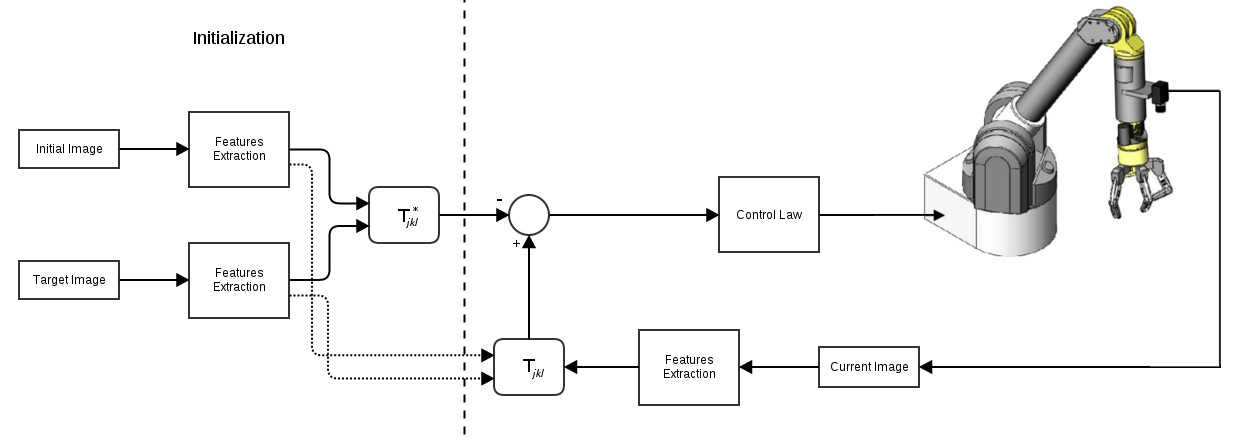
\includegraphics[width=150mm,height=70mm]{figures/vsttloop.png}
  \caption{Block diagram of the proposed Trifocal Tensor Visual Servoing loop control}
  \label{fig:vsttloop}
\end{figure}

In Figure~\ref{fig:vsttloop}, we present the block diagram explaining the proposed trifocal tensor visual servoing control loop. At initialization, the desired tensor $T_{(jkl)}^{*}$ is computed from feature correspondences across three images obtained from the three camera poses: initial pose, desired pose, and current pose being equal to the desired pose. In this method, we assume the camera intrinsic parameters are known. It means before computing the tensor from image correspondences, matching points have to be transformed to calibrated coordinates.

The current tensor $T_{(jkl)}$ is computed inside the visual servoing loop at each iteration. Then the interaction matrix is computed using the current tensor. For simplicity, we make the assumption that the initial pose is known and the interaction matrix can be computed directly. The new error value is computed along with the pseudo-inverse of the interaction matrix and fed back to the control law to compute the required velocities to drive the camera to the desired pose. The system converges and the loop is terminated when the camera reaches the desired pose. This is evaluated when the sum squared of the error reaches a value less than a defined threshold, $1 \times \e{-6}$ for example.
